\vspace{-2mm}
\section{Introduction}
\vspace{-2mm}
\label{sec:intro}

% \begin{itemize}
%     \item  Problem to solve using your work (Motivation). Why is it important/of value?
%     \item Brief story of the solutions for the problem to solve 
%     \item From the related work principles on which the papers are based arrive to the SoTA baselines.  (Place related work points here if section isn't in format)
%     \item Introduce the research gap that our work will fill. How our solution contrasts to other solutions or partial solutions to this gap. 
%     \item State the contribution of the work.
% \end{itemize}

% Robot Foundation Model
% Problem to solve: towards a robot foundation model that is able to control any kind of robot embodiment. Explain the importance and the necessity of a robot foundation model, how it will make it possible to do a bunch of things.


% Cross embodiment learning introduction and SotA
% The current SotA robot models can reliably perform various tasks in the real world, nonetheless, they are bound to the type of control and the embodiment of the robot (Add references to SoTA robot control, explain a couple of examples of how this is done). 

% Papers on cross embodiment learning. Current publications on cross-embodiment learning use a: encoder decoder method, etc. that still require a prior knowledge and data of the current robot hand to use in order to generalize task knowledge across different robot embodiments. 

% If we would like to add a new robot we would need to retrain the entire model from scratch, wasting resources, time and requiring an immense amount of new data. 

% Latent Space representations for transfer, state disadvantages of the space created by encoders. 



% Data Collection Disadvantege
% Human data problem: Robot learning requires a lot of resources to train in the case of simulation RL. In the case of imitation learning it requires a lot of data which suffers the same problem of not being able to reuse with different embodiments. If the data is obtained by controlling the robot itself, it's capture requires huge amount of time, is cumbersome, and can be suboptimal given that every demonstrator would need to train on how to control the robot and then perform the tasks correctly. Furthermore, if the data is taken from human demonstrations the translation to robot actions is not trivial, human hands differ greatly in proportion and size, which creates a lot of errors in the translation which then affect the training and performance of the models.

% Intermediate Grasp representations in Robotic Grasping



% Introduction of our method
% In this paper we present the Universal Gripper Action Space (UGAS), a method able to generalize actions across different robot hands. We take inspiration on the robotic grasp generation problem where multiple intermediate grasp representations have been developed to allow the generation models to generalize across grippers.

% - CORL double blind reviews - need to remove this reference to our work.

% Specifically we base this approach on our previous work "RobotFingerPrint", where we create a intermediate grasp representation with dense correspondences between every robot gripper and a "maximal sphere". 

% Torwards a foundation model that can learn from and control any embodiment. 



% % Snippet of what is good in this paper
% We test our method using the common task of reposing the DexCube (cite NVIDIA paper) using Isaac Lab. We were able to achieve high zero-shot cross embodiment performance. 

Robot manipulation has made rapid progress in recent years due to advances in imitation learning~\cite{zhao2023learning,chi2025diffusion}, reinforcement learning~\cite{kalashnikov2018scalable,singh2024dextrah}, and vision-language-action (VLA) models~\cite{kim2024openvla,black2024pi0visionlanguageactionflowmodel,intelligence2025pi05}. While recent policies have demonstrated impressive capabilities in grasping, pick-and-place, dexterous manipulation, and long-horizon task execution, most large-scale robot learning systems and datasets remain dominated by relatively simple end-effectors such as parallel-jaw grippers~\cite{brohan2022rt1,brohan2023rt2visionlanguageactionmodelstransfer,team2024octo,o2024open,khazatsky2024droid}. In contrast, dexterous robotic hands remain comparatively underexplored due to their highly diverse kinematic structures, action parameterizations, and control interfaces. As a result, existing dexterous manipulation systems often rely on embodiment-specific action spaces, datasets, and retraining procedures~\cite{wen2025grdextertechnicalreport,zhang2026dexora,zheng2026egoscale}, making cross-embodiment transfer across robotic hands challenging.




To address this challenge, we investigate the problem of robot learning in a unified hand action space for robot manipulation. \emph{The central idea of our approach is to represent hand actions through the deformation of a canonical sphere representation.} Instead of defining actions directly in embodiment-specific joint spaces, we model manipulation actions as geometric deformations on a shared spherical surface. This representation provides a continuous and embodiment-agnostic interface that captures the semantic behavior of robotic hands while abstracting away low-level hardware differences.

Our sphere-based action representation is motivated by the observation that many robotic hands interact with objects through spatial contact patterns around an object-centered workspace despite their diverse mechanical designs. By representing hand actions as deformations of a canonical sphere, we obtain a shared geometric action space that generalizes across different hand morphologies. Embodiment-specific hand motions are recovered through the proposed inverse kinematics algorithm that maps sphere deformations to executable joint configurations. This unified representation enables cross-embodiment policy transfer, data sharing across heterogeneous robotic platforms, and scalable policy learning for future robot foundation models. 


\begin{figure}
 \centering 
 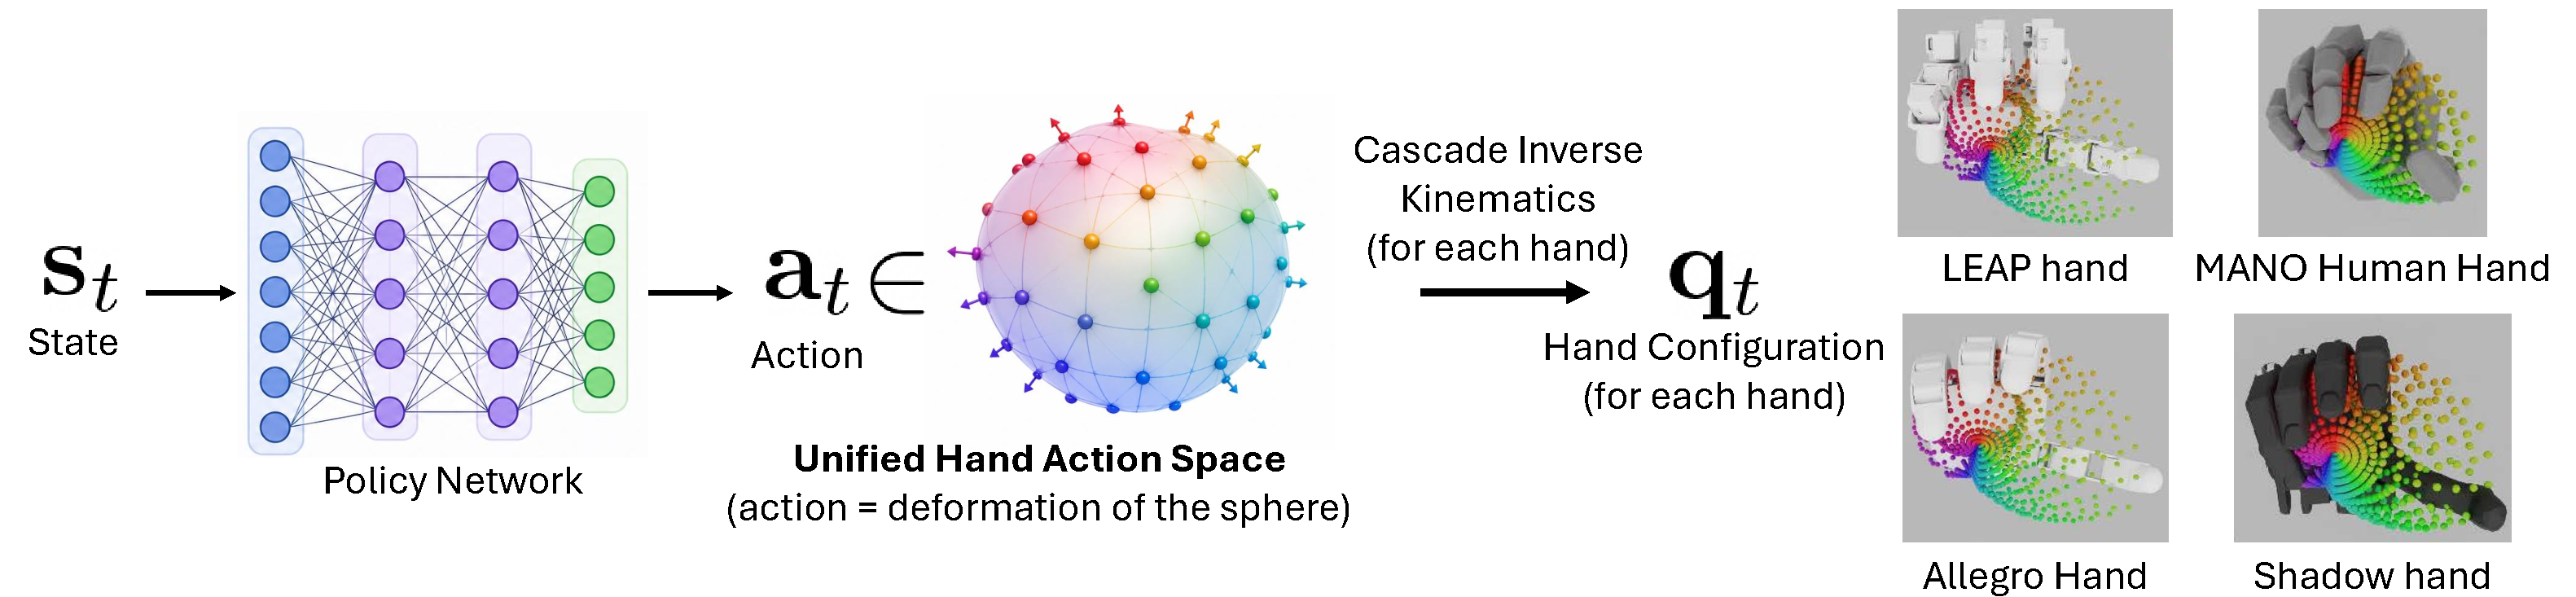
\includegraphics[width=\textwidth ]{figures/intro.pdf}\vspace{-3mm}
   \caption{In our unified hand action space, an action is represented as the deformation of a canonical sphere. A deformed sphere is mapped to hand configurations of various embodiments (LEAP~\cite{shaw2023leaphand}, Allegro~\cite{allegrohand}, MANO Human~\cite{MANO:SIGGRAPHASIA:2017} and Shadow~\cite{shadowhand}).}      
   \label{fig:intro}
   \vspace{-4mm}
\end{figure}

In this work, we build upon the proposed sphere-based unified hand action space to develop a framework for cross-embodiment dexterous manipulation. We introduce a geometric action representation based on sphere deformations together with a cascade inverse kinematics algorithm that maps the unified representation to embodiment-specific hand joint configurations. Using reinforcement learning~\cite{schwarke2025rslrl}, we train manipulation policies directly in the proposed action space for dexterous in-hand manipulation. We evaluate our method on in-hand cube reorientation tasks across multiple robotic hands with different kinematic structures. Experimental results demonstrate that the proposed representation enables stable dexterous control, effective multi-hand policy learning, and meaningful zero-shot transfer to previously unseen robotic hands. The main contributions of this work are:
\begin{itemize}
    \vspace{-2mm}
    \item We propose the Unified Hand Action Space (UHAS), a sphere-based geometric action representation that models robotic hand actions as deformations of a canonical sphere.
    
    \item We develop a Cascade Inverse Kinematics (CIK) algorithm that maps the unified sphere representation to heterogeneous robotic hands with different kinematic structures.
    
    \item We demonstrate dexterous in-hand manipulation, multi-hand policy learning, and cross-embodiment transfer across multiple robotic hands in simulation and the real world, including zero-shot transfer to unseen hands.
\end{itemize}




